\title{Anisotropic Thermal Conductivity of Cermet Nuclear Waste}
\author{} \institute{}
\tocauthor{\underline{V.~F.~de~Almeida}, C.~Ausmus, R.~T.~Jubin, P.~Solin}
\maketitle

\begin{center}
{\large \underline{Valmor F. de Almeida}, Clint Ausmus, and Robert T. Jubin}\\
Oak Ridge National Laboratory {\tt dealmeidav@ornl.gov}\\
\vspace{4mm}

{\large Pavel Solin}\\
University of Nevada {\tt solin@unr.edu}
\end{center}

\section*{Abstract}
Cermet is a microscopically heterogeneous material by design wherein a  ceramic phase coexists with a metal phase. One of the objectives of this combination is to improve heat removal from the  ceramic phase in this nuclear waste form. The purpose of this work is to develop methods to predict effective thermal conductivity coefficients from knowledge of the microstructure of the material. This transport property is required in coarser continuum models for thermo-mechanics of cermet material bodies. This work describes the use of hp-adaptivity using HERMES-2D in two disparate applications that share the same mathematical framework. In one application, a heat-conduction-like equation is used in the image processing of cermet elemental maps obtained with scanning electron microscopy (SEM) to identify solid phases. In the other application, a corresponding multi-phase, micro-continuum heat conduction equation is solved to obtain the temperature field which provides the means for deriving an averaged thermal conductivity tensor. Results show that a cylindrical pellet of cermet nuclear waste  may experience higher heat flux in the radial direction by as much as 30\% when compared to the axial direction. In addition, results suggest that the material is nearly orthotropic and they demonstrate that simple volume fraction average overestimates heat conduction.

\begin{figure}
\centering
\begin{tabular}{cccc}
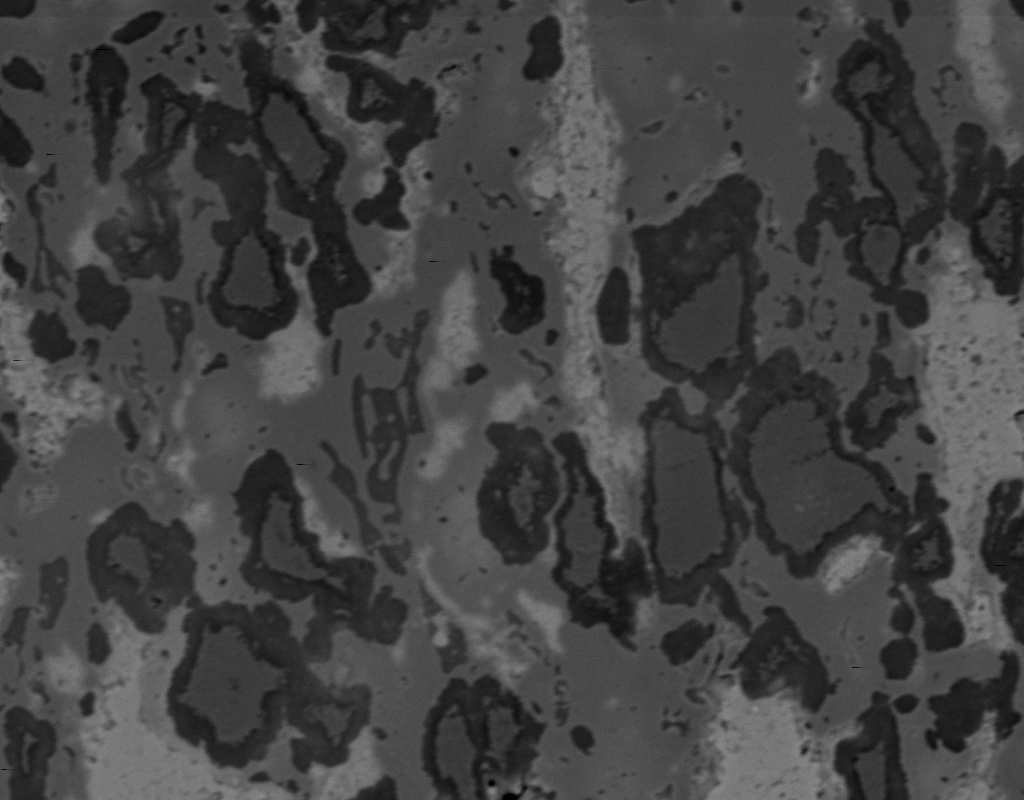
\includegraphics[height=0.9in]{./almeida/cermet-SEM.png} &
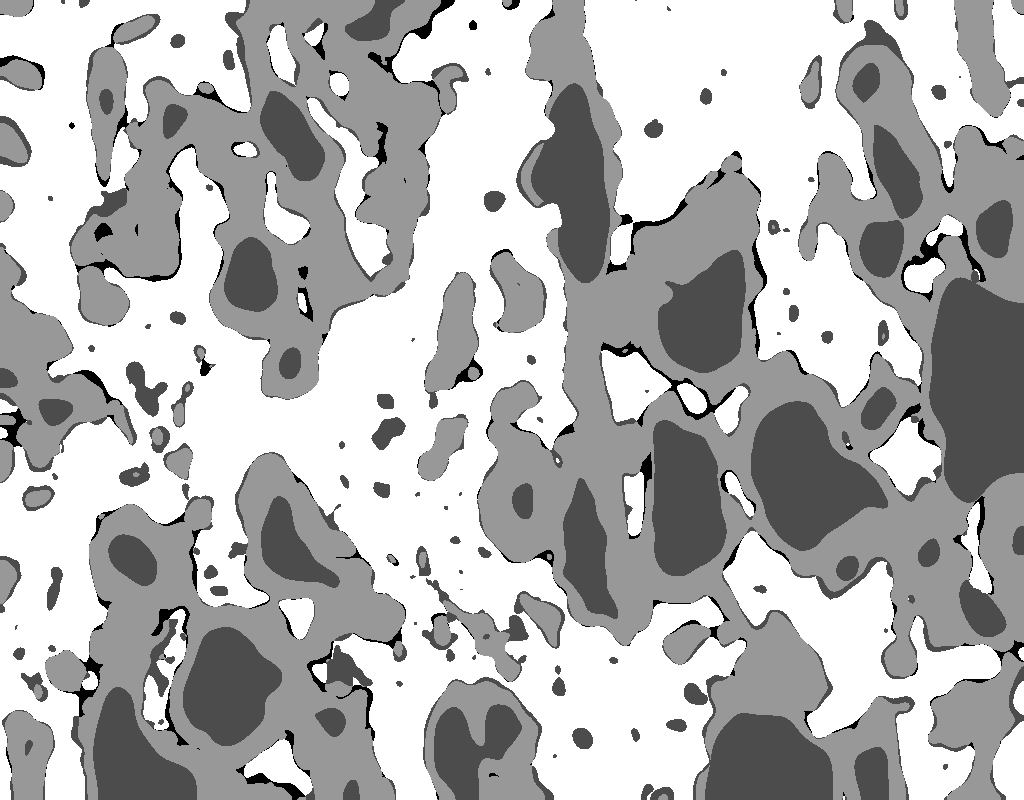
\includegraphics[height=0.8in]{./almeida/cermet-phases.png} &
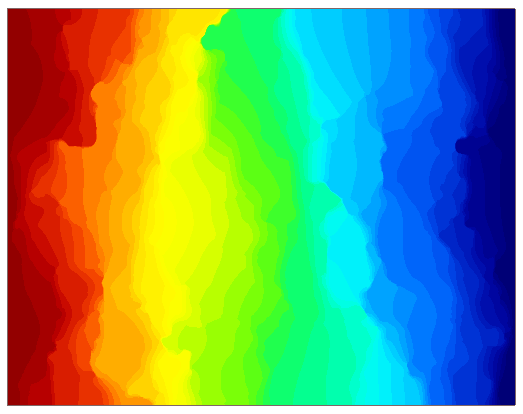
\includegraphics[height=0.8in]{./almeida/cermet-xtfield.png} &
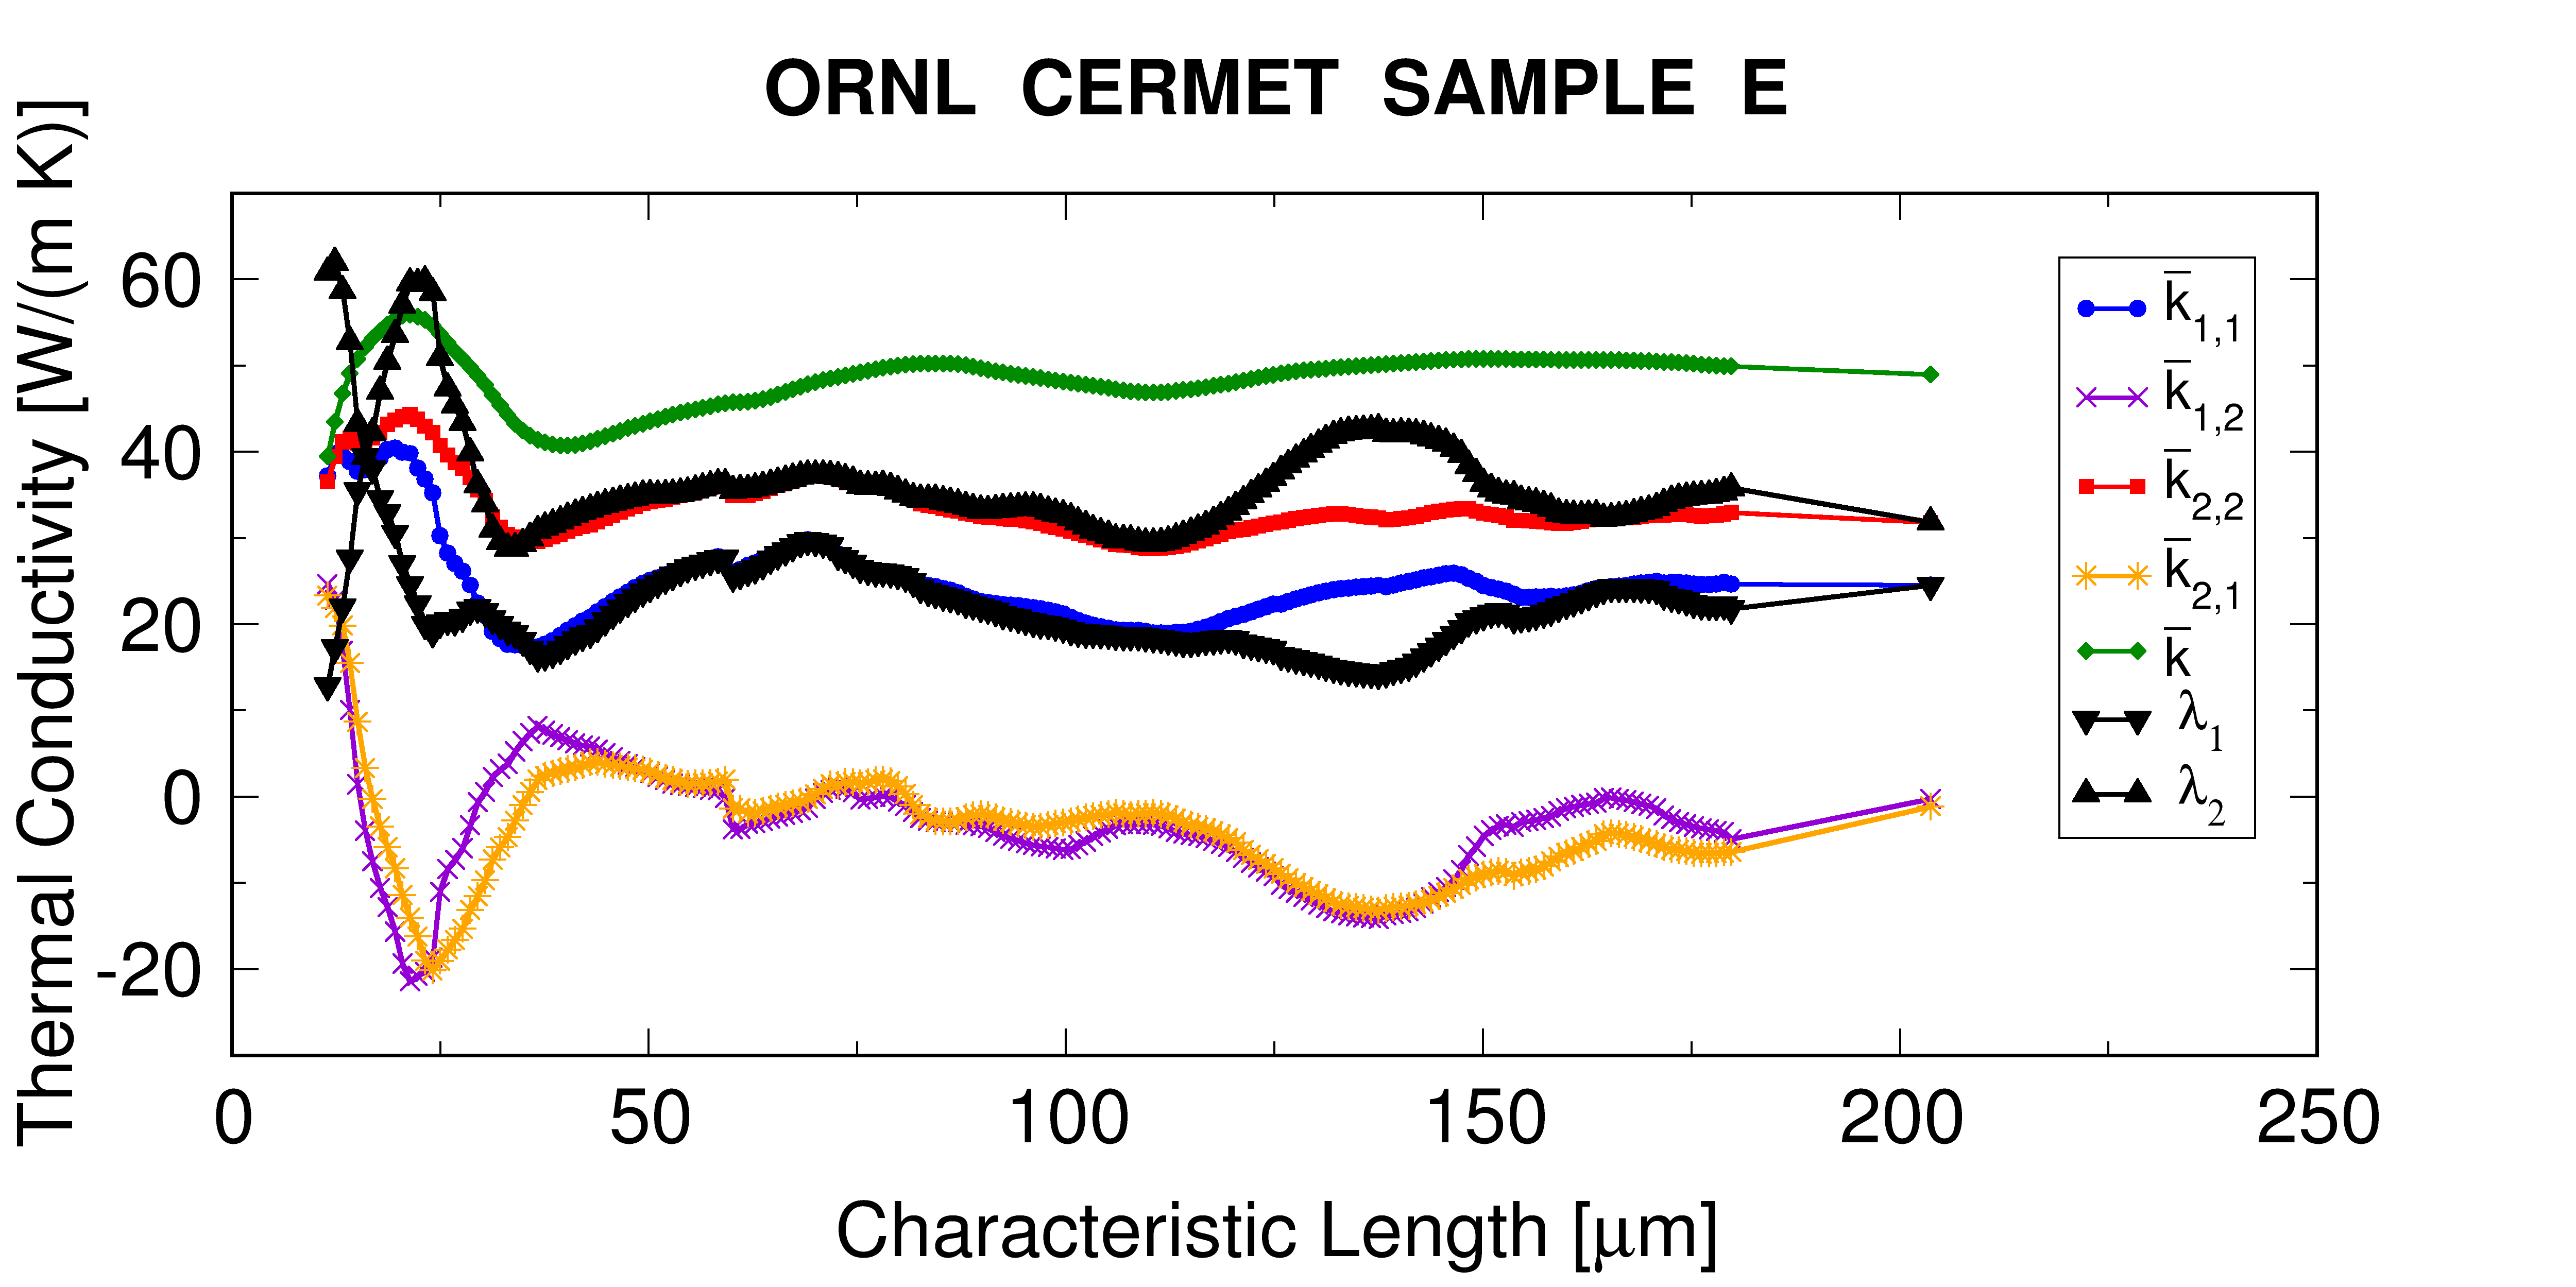
\includegraphics[height=0.8in]{./almeida/cermet-ktensor.png}
\\
(a) & (b) & (c) & (d)
\end{tabular}

\caption[Anisotropic thermal conductivity of cermet nuclear waste]{Main steps for computing the effective thermal conductivity tensor of a cermet waste form. \textbf{(a)} SEM image at origin of $z$--$r$ plane of pellet (${230x180\mathrm{\mu}m}^{2}$). \textbf{(b)} Multiphase segmentation using non-linear, inhomogeneous, anisotropic diffusion. \textbf{(c)} Temperature field when the sample is heated horizontally (a similar realization is applied vertically). \textbf{(d)} Averaging length scale variation of the derived thermal conductivity tensor components $\kappa_{i,j}$, eigenvalues $\lambda_i$, and volume fraction average conductivity $\overline{\kappa}$.}
\end{figure}

\bibliographystyle{plain}
\begin{thebibliography}{10}
\bibitem{jubin-etal-11}
{\sc R.T.~Jubin \emph{et al.}}. {Development of advanced cermet waste forms}. Waste Management Conference 2011, February 27--March 3, Phoenix, AZ.
\end{thebibliography}
